\documentclass[12pt]{article}

\usepackage{fullpage}
\usepackage{multicol,multirow}
\usepackage{tabularx}
\usepackage{ulem}
\usepackage[utf8]{inputenc}
\usepackage[russian]{babel}
\usepackage{listings}
\usepackage{hyperref}
\usepackage{graphicx}
\DeclareGraphicsExtensions{.png}


\begin{document}

\section*{БЖД}

Выполнила студентка группы М8О-407Б \textit{Довженко Анастасия}.

\subsection*{Теория 1}
\begin{itemize}
\item Что значит "КЕО характеризует освещённость точек помещения"?

КЕО --- выраженное в процентах отношение освещённости в данной точке внутри помещения (ЕВН) к одновременному значению наружной горизонтальной освещённости, создаваемой светом полностью открытого небосвода (ЕНАР).

\item Почему для нормирования естественного освещения используется КЕО?

КЕО оценивает размеры оконных проёмов, вид остекления и переплётов, их загрязнение, то есть способность системы естественного освещения пропускать свет. Естественное освещение характеризуется тем, что создаваемая освещённость изменяется в чрезвычайно широких пределах в зависимости от времени дня, года, метеорологических факторов. Поэтому естественное освещение невозможно количественно задавать величиной освещённости. В качестве нормируемой величины для естественного освещения принята относительная величина – коэффициент естественной освещённости (КЕО).

\item Светоотдача у каких лам больше?

Самой большой светоотдачей обладают газоразрядные лампы.

\item Возможно ли использовать для наружного освещения люминисцентные лампы и почему?

Для некоторых видов люминесцентных ламп существуют ограничения по температуре окружающей среды (при температурах, близких к 0 градусам), следовательно, их использовать невозможно.

\item Определить требуемую величину искусственного освещения для : 1) работ в литейном цехе; 2) выполнения чертёжных работ (с указанием ссылки на нормативный документ).

Нормативный документ --- СНиП 23-05-95
Литейный цех --- 36лк.
Чертёжные работы --- 1250лк-5000лк.

\item В чём отличие общего локализованного освещения от местного?

Общее освещение – это освещение, при котором светильники размещаются в верхней зоне помещения. Светильники могут быть расположены равномерно или применительно к расположению оборудования или рабочих мест.

\item В каких случаях для расчёта искусственного освещения применяется точечный метод, а в каких метод светового потока?

Точечный метод применяется в случае, если свет, отражённый от стен и потолка не имеет большого значения, например, в цехах с крупногабаритным оборудованием и т.д.. Метод светового потока более сложен и учитывает отражения от стен, потолка и других поверхностей. 

\item  С чем связано недостаточное значение КЕО в зданиях?

Недостаточное значение КЕО в знаниях связано с небольшим количеством естественного освещения внутри зданий. Кроме того, причиной может служить тёмная окраски интерьера (от тёмных цветов свет отражается хуже, чем от светлых)

\end{itemize}

\subsection*{Теория 2}
\begin{itemize}

\item Почему шум нормируется показателем "уровень звукового давления" (дБ), а не "звуковое давление" (Па)?

Слух человека способен реагировать на прирост звукового давления, шум нормируется исходя из отношения звукового давления или интенсивности звука в точке к соответствующему пороговому значению.

\item В чем отличия единиц измерения дБ и дБА? Какая взаимосвязь между методом нормирования по предельному спектру и эквивалентному уровню?

ДБА – уровень звукового давления шума в нормируемом диапазоне частот, корректированный по частотной характеристике А шумомера. 
при нормировании шума используют 2 метода: нормирование по предельному спектру шума и интегральная оценка.
Первый метод нормирования является основным для постоянных шумов. Здесь нормируются уровни звуковых давлений в восьми октавных полосах. Совокупность допустимых уровней звукового давления в восьми октавных полосах частот называется предельным спектром. Причём, с ростом частоты допустимые уровни уменьшаются.
Интегральная оценка применяется для нормирования непостоянных шумов и в тех случаях, когда не известен спектр реального шума. Нормируемым показателем в этом случае является эквивалентный уровень звука широкополосного постоянного шума, оказывающий на человека такое же влияние, как и реальный непостоянный шум, измеряемый по шкале А шумомера. При этом нормируемая величина измеряется в дБА.

\item В каких случаях нормирование осуществляется только в дБА?

В тех случаях, когда не известен спектр реального шума.

\item Определить уровень шума от точечного источника на расстоянии 8м и 64м, если на расстоянии 2 м уровень шума составляет 80 дБА?

На расстоянии 8м -- 68 дБА, на расстоянии 8м -- 50 дБА

\item Определить уровень шума от плоскостного источника размерами (200м х150м), на расстоянии 50 м и 100м,  если на расстоянии 25 м уровень шума равен 82 дБА?

На расстоянии 50м -- 82 дБА, на расстоянии 100м -- 79 дБА

\item Эффективность акустического экрана на частоте 1000Гц составляет 18,35 дБ, а на частоте 2000 Гц = 16,48 дБ, размеры экрана hxl=1.2x1.4 м. определить на каком расстоянии от источника шума установлен экран (a), если расстояние от экрана до рабочего места (b) составляет 1,3 м?

Экран установлен на расстоянии 0.16 м.

\end{itemize}


\subsection*{Задача 2, вариант 6}

Рассчитать общеобменную вентиляцию в цехе (на участке) Х, обеспечивающую требуемое состояние воздушной среды при условии одновременной работы всех Y работников и выделении в воздух вредного вещества Z. Температура воздуха в помещении 21ºС. Исходные данные для расчёта массы, выделяющихся вредных веществ на малярном участке, количество рабочих мест 4, вредные вещества сольвент. Применяемый лакокрасочный материал Шпаклёвка ПФ-002, расход лакокрасочных материалов на единицу площади изделия 1000.

ПДК Сольвент = 100 мг/м\^3

$C_{n} = 0$

$L_1 = m/$(ПДК - $C_{n}$) = $10aqm$/(ПДК - $C_{n}$)

$a = 12$ м2/ч -- производительность одного рабочего дня

$q = 1000$ г/м2 -- расход лакокрасочных материалов на единицу площади изделия

$m = 25\%$ -- содержание летучих компонентов в краске.

$L_1 = 30000$ м3/ч

$L_M = \sum_{i=1}^{4}L_{M_{i}} = 4L_{i} = 120000$ м3/ч

Скорость движения воздуха в воздуховоде на участке I: $v_{1} = 12$ м/с

$d_{1} = 0.033 \sqrt{\frac{L_1}{v_1 \pi}} = 0.931$ м

$d_{1}^' = 0.9$ м

$v_{1}^' = \frac{0.033^{2}L_1}{\pi d_{1}^{'2}} = 12.838$

$\ro = \frac{353}{273+t} = 1.201$

$\lambda = 0.02$

Диаметры воздуховодов для $II, III, IV$ участков $d_i = \frac{d_{i-1}^'}{0.7}$

Сопротивление движению воздуха на каждом участке: 
$H = \frac{\ro  v_{1}^{'2}}{2}(\lambda \frac{1}{d^'} + \sum_{i=1}^{n}\epsilon_{M_{i}})$

Общее сопротивление движению воздуха на каждом участке:
$H_{C} = \sum_{i=1}^{m} H_{i} = 1006$

$k = 1.1$

$L_{B} = L * k = 120000 * 1.1 = 132000$

Выбираем вентилятор В-Ц4-76 №20 с диаметром рабочего колеса 2м с КПД 84%

Частота вращения электродвигателя 1470 мин-1, мощность 75 кВт

\subsection*{Задача 7, вариант 6}

Определить уровень звукового давления на рабочем месте шлифовальщика, если в цехе расположено 3 токарных станка, 3 фрезерных и 2 шлифовальных. Расстояние от рабочего места, на котором необходимо определить уровень шума, до токарных станков 5м, 6м и 8.2м, до фрезерных станков 2.55м, 4.25м, 7.3м, до шлифовальных станков 1м и 4.9м. Исходные данные для решения задачи приведены в таблицах 4.10 – 4.13.

Размеры цеха $a x b x h = 9 x 6.5 x 4.2$ , в стене протяжённостью 9м расположено 4 окна, размерами $a x b = 1.8 x 2.4$. При расчётах принимать, что стены цеха из кирпича, а пол и потолок из бетона.

В помещении планируется выполнить звукопоглощение. Рассчитать эффективность применения данного метода защиты материалом

Определение площади ограждающих поверхностей

S пола = 58.5 м2

S стен = 130.2 м2

S окон = 17.28 м2

S огр = 2S пола + S стен - S окон = 229.92 м2

S облицовки = S потолка + S cтен - S окон - S облицовки = 171.72 м2

S огр, без облицовки = 2S пола + S стен - S окон - S облицовки = 58.2 м2

Расстояние от расчётной точки до акустического центра ближайшего источника шума $r_{min} = 1$ м

$5r_{min} = 5$м. На расстоянии до 5м находятся 1 токарный станок, 2 фрезерных станка и 2 шлифовальных станка, все остальные источники находятся на большем расстоянии.


Так как измерение уровня шума производится на рабочем месте шлифовальщика (то есть непосредственно возле станка), из таблицы допускаемых уровней звукового давления в октавных полосах частот ГОСТа 12.01.003-83 выберем пункт 5.

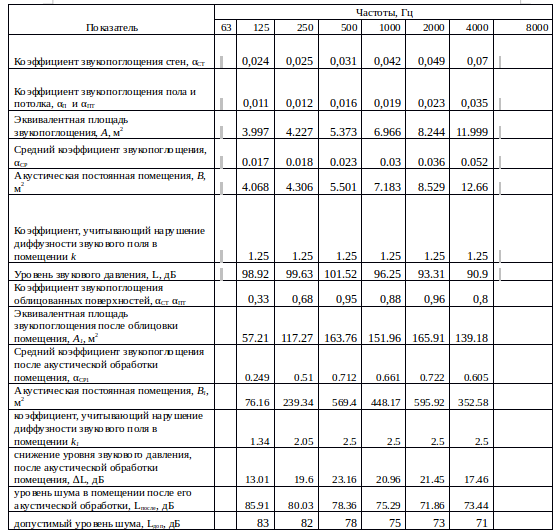
\includegraphics[width=\linewidth]{2.png}\\

На октавных полосах частот 250Гц и 2000Гц акустическая обработка данным материалом обеспечивает уровень шума ниже допустимого, а на 1000Гц находится на уровне нормы в пределах погрешности. На низких высоких частотах снижение шума недостаточно и необходима дополнительная обработка или использование других средств защиты. 

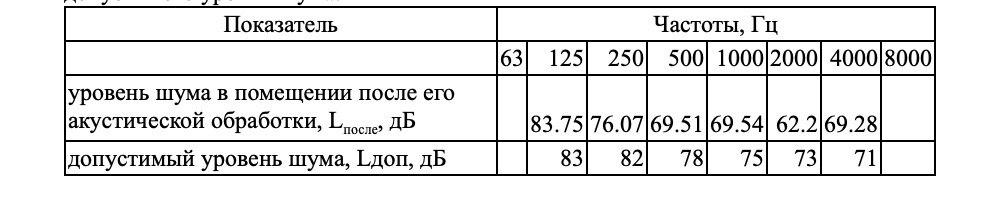
\includegraphics[width=\linewidth]{1.jpg}\\

\end{document}
